%%%%%%%%%%%%%%%%%%
% Based on https://github.com/jdavis/latex-homework-template
%%%%%%%%%%%%%%%%%%

\documentclass{article}

\usepackage{fancyhdr}
\usepackage{extramarks}

\usepackage{amsmath}
\usepackage{amsthm}
\usepackage{amsfonts}

\usepackage{tikz}
\usepackage[plain]{algorithm}
\usepackage{algpseudocode}

\usepackage{wrapfig}

\usepackage{lipsum}

%for urls
\usepackage{hyperref}
\hypersetup{
	colorlinks = true,
	linkcolor = teal,
	anchorcolor = teal,
	citecolor = teal,
	filecolor = teal,
	urlcolor = teal
}

%%%%%% Basic Document Settings %%%%%%%%%

\topmargin=-0.45in
\evensidemargin=0in
\oddsidemargin=0in
\textwidth=6.5in
\textheight=9.0in
\headsep=0.25in

\linespread{1.1}

%%%%%%%%%%%%%%%%%% Homework Details %%%%%%%%%%%%%%%
% University Logo
% Title
% Due date
% University
% Class
% Instructor
% Author
% Author ID 
\newcommand{\hmwkSeal}{images/logo.png}
\newcommand{\hmwkTitle}{Assignment \#4}
\newcommand{\hmwkDueDate}{Jan 6, 2023}
\newcommand{\hmwkClass}{Introduction to Artificial Intelligence (CS-487) }
\newcommand{\hmwkClassInstructor}{Professor I. Tsamardinos}
\newcommand{\hmwkUniversity}{University of Crete \\Department of Computer Science}
\newcommand{\hmwkAuthorName}{Nikolaos Kougioulis}
\newcommand{\hmwkAuthorID}{ID 1285}


%fancyhdr
\pagestyle{fancy}
\lhead{\hmwkAuthorName\ (\hmwkAuthorID)} %left head
%\chead{\hmwkClass\ \hmwkTitle} %center head
%\rhead{\date{\today}} %right head
\rhead{\hmwkClass\ \hmwkTitle} 
\lfoot{\lastxmark}
\cfoot{\thepage}

\renewcommand\headrulewidth{0.4pt}

% Create Problem Sections %

\newcommand{\enterProblemHeader}[1]{
	\nobreak\extramarks{}{Problem \arabic{#1} continued on next page\ldots}\nobreak{}
	\nobreak\extramarks{Problem \arabic{#1} (continued)}{Problem \arabic{#1} continued on next page\ldots}\nobreak{}
}

\newcommand{\exitProblemHeader}[1]{
	\nobreak\extramarks{Problem \arabic{#1} (continued)}{Problem \arabic{#1} continued on next page\ldots}\nobreak{}
	\stepcounter{#1}
	\nobreak\extramarks{Problem \arabic{#1}}{}\nobreak{}
}

\setcounter{secnumdepth}{0}
\newcounter{partCounter}
\newcounter{exerciseCounter}
\setcounter{exerciseCounter}{1}
\nobreak\extramarks{Problem \arabic{exerciseCounter}}{}\nobreak{}

% Homework Problem Environment %
% This environment takes an optional argument. When given, it will adjust the problem counter. This is useful for when the problems given for your
% assignment aren't sequential. See the last 3 problems of this template for an example.
%

\newenvironment{Exercise}[1][-1]{
	\ifnum#1>0
	\setcounter{exerciseCounter}{#1}
	\fi
	\section{Exercise \arabic{exerciseCounter}}
	\setcounter{partCounter}{1}
	\enterProblemHeader{exerciseCounter}
}{
	\exitProblemHeader{exerciseCounter}
}

% Title Page %
\title{
	\centering
	\includegraphics[height=1.5in]{\hmwkSeal}
	
	\vspace{1in}
	\textmd{\textbf{\hmwkClass\ \hmwkTitle}}\\
	
	\normalsize\vspace{0.1in}\small{Due\ on\ \hmwkDueDate}\\
	
	\vspace{0.1in}
	\large{\textit{\hmwkClassInstructor}} \\
	\vspace{0.5in}
	
	\large{\hmwkUniversity}
	
	\vspace{3in}
	
	\author{\textbf{\hmwkAuthorName} (\hmwkAuthorID)}
	\date{\today}
}

% Various Helpers %
\newcommand{\alg}[1]{\textsc{\bfseries \footnotesize #1}}
% For derivatives
\newcommand{\deriv}[1]{\frac{\mathrm{d}}{\mathrm{d}x} (#1)}
% For partial derivatives
\newcommand{\pderiv}[2]{\frac{\partial}{\partial #1} (#2)}
% Integral dx
\newcommand{\dx}{\mathrm{d}x}
\newcommand{\E}{\mathbb{E}}
\newcommand{\Var}{\mathrm{Var}}
\newcommand{\Cov}{\mathrm{Cov}}
\newcommand{\Bias}{\mathrm{Bias}}

\def\code#1{\texttt{#1}}

%for code listings
\usepackage{listings}
\usepackage{xcolor}

\definecolor{codegreen}{rgb}{0,0.6,0}
\definecolor{codegray}{rgb}{0.5,0.5,0.5}
\definecolor{codepurple}{rgb}{0.58,0,0.82}
\definecolor{backcolour}{rgb}{1,1,1}

\lstdefinestyle{mystyle}{
	backgroundcolor=\color{backcolour},   
	commentstyle=\color{codegreen},
	keywordstyle=\color{magenta},
	numberstyle=\tiny\color{codegray},
	stringstyle=\color{codepurple},
	basicstyle=\ttfamily\footnotesize,
	breakatwhitespace=false,         
	breaklines=true,                 
	captionpos=b,                    
	keepspaces=true,                 
	numbers=left,                    
	numbersep=5pt,                  
	showspaces=false,                
	showstringspaces=false,
	showtabs=false,                  
	tabsize=2
}

\lstset{style=mystyle}

\begin{document}

	\maketitle
	
	\pagebreak
	
Many problems in the field of Artificial Intelligence are reduced to finding a path on a graph. We can represent a directed graph in Prolog (like the one in Figure 1a) using the following facts: \\

\begin{center}
\code{connect(a, b).} \\
\code{connect(b, c).} \\
\code{connect(b, d).} \\
\code{connect(e, d).} \\
\code{etc …} \\
\end{center}
		
\begin{wrapfigure}{r}{0.3\textwidth}
	\begin{center}
		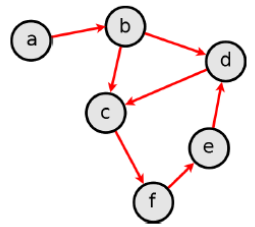
\includegraphics[width=0.2\textwidth]{images/fig1a.png}
	\end{center}
	\caption{A directed graph.}
		\begin{center}
		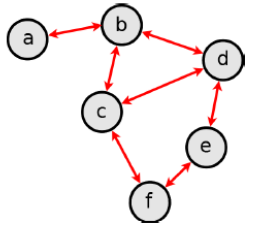
\includegraphics[width=0.2\textwidth]{images/fig1b.png}
	\end{center}
	\caption{A non-directed graph.}
\end{wrapfigure}

A simple way to represent a non-directed graph (like the one in Figure 2) would be to double the number of facts to state all the reverse connections (e.g. \code{connect(b, a)} ). A better way is to define the following two rules: \\

\begin{center}
	\code{interconnected(X, Y):- connect(X, Y).} \\
	\code{interconnected(X, Y):- connect(Y, X).} \\
\end{center}

where the predicate \code{interconnected/2} represents the bi-directional relationship between the nodes. \vspace{30ex} 
	
	\begin{Exercise}Could we use just one rule like the following (instead of two rules)? \begin{center} \code{interconnected(X, Y):- interconnected(Y, X).} \end{center} Explain your answer. Are there situations where the above rule would work and other situations that would be problematic? \\
	\end{Exercise}

    \textbf{Solution:} \\
    
    Using just the above symmetric rule, 
    
    \code{interconnected(X, Y):- interconnected(Y, X).} \\
    
    instead of two (\code{interconnected(X, Y):- connect(X, Y), connect(Y, X).}), is mostly problematic and cumbersome compared to the rule used at the beginning of the text. \\
    
    \begin{figure}
    	\centering
    	\begin{minipage}{0.45\textwidth}
    		\centering
    		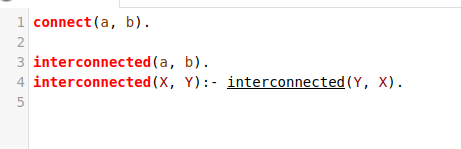
\includegraphics[width=0.9\textwidth]{images/ex1_input} 
    		\caption{Exercise 1: A knowledge base of rules in the SWISH environment of SWI-Prolog.}\footnote{\url{https://swish.swi-prolog.org/}} 
    		\label{ex1.0}
    	\end{minipage}\hfill
    	\begin{minipage}{0.55\textwidth}
    		\centering
    		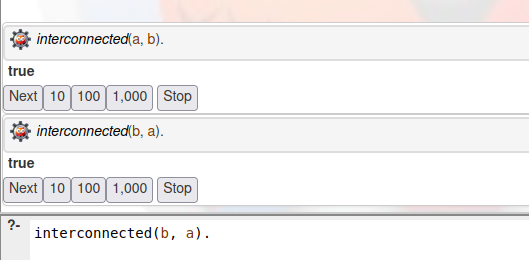
\includegraphics[width=0.9\textwidth]{images/ex1_output}
    		\caption{Successfully querying \code{?- interconnected(a, b).} and \code{?- interconnected(b, a)}.}
    		\label{ex1.1}
    	\end{minipage}
    \end{figure}
    
    Consider a graph with two nodes, $a$ and $b$. If \code{connect(a, b).} and \code{interconnected(a, b).} exist in our Knowledge Base, then by performing the query \code{?- interconnected(a,b)} we obviously obtain \code{true}, as it already exists in our Knowledge Base. Querying \code{?- interconnected(b,a)} we also obtain \code{true}, as it is derived using Modus Ponens from the \code{interconnected} rule (Figures 3 \& 4). \\
    
    Now consider the case our KB contains only the rules \code{connect(a,b).}, \code{connect(b,a).}, and \code{interconnected(X, Y):- interconnected(Y, X).} (Figures 5 \& 6). From the first two rules, it is evident that if a is connected to b and b is connected to a means \code{interconnected(a,b)} and \code{interconnected(b,a)} yield \code{true}. This however is not entailed and logically derived from our KB, so such queries would fail. 

    \begin{figure}
	\centering
	\begin{minipage}{0.45\textwidth}
		\centering
		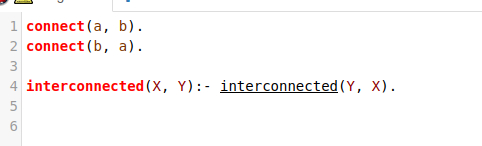
\includegraphics[width=0.9\textwidth]{images/ex1_0_input} 
		\caption{Exercise 1: Altered Knowledge Base.}
		\label{ex1.2}
	\end{minipage}\hfill
	\begin{minipage}{0.45\textwidth}
		\centering
		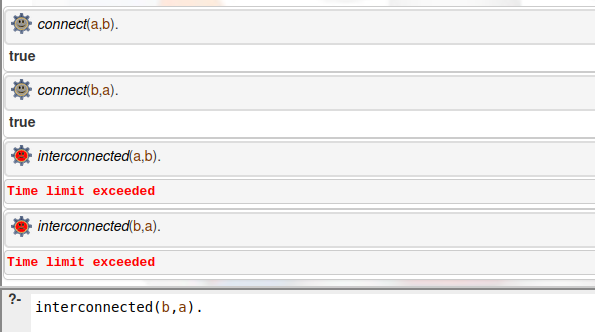
\includegraphics[width=0.9\textwidth]{images/ex1_0_output} 
	   \caption{Exercise 1: Example of unsuccessful KB Query.}
	   \label{ex1.3}
	\end{minipage}
    \end{figure}


    \newpage
    
    \begin{Exercise}Define a predicate \code{exists\textunderscore path/2} that implements a simple Depth-First Search. This predicate just confirms the existence of a connection between two nodes. For example, the following question would answer "true":
    	
    	\code{?- exists\textunderscore path(a, f). \\
    		true} \\
    	
    \end{Exercise} 

    \textbf{Solution}\\
    
    The solution is based on the recursive definition of the path from Graph Theory as follows: 
    
    \begin{lstlisting}[language=Prolog]
%exists_path/2
exists_path(StartNode, EndNode).
exists_path(StartNode, EndNode) :- interconnected(StartNode, NextNode),
                                exists_path(NextNode, EndNode).
    \end{lstlisting}

        \begin{figure}
    	\centering
    	\begin{minipage}{0.55\textwidth}
    		\centering
    		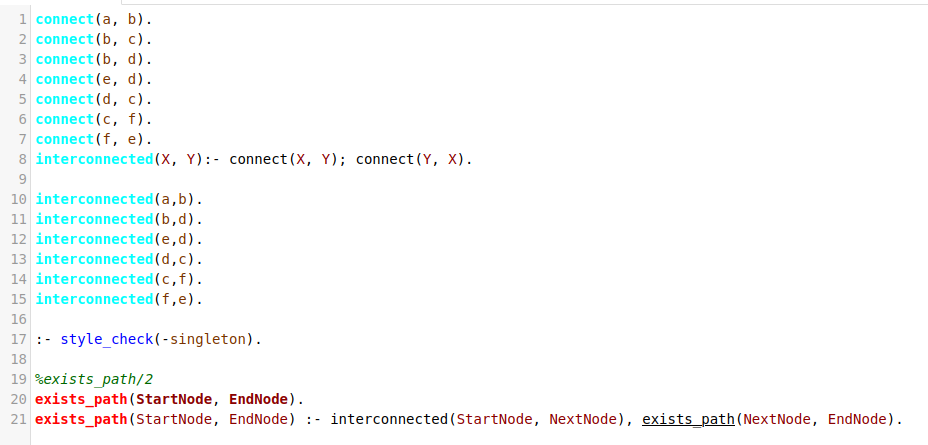
\includegraphics[width=0.9\textwidth]{images/ex2_input} 
    		\caption{KB and rules in Exercise 2.}
    	\end{minipage}\hfill
    	\begin{minipage}{0.45\textwidth}
    		\centering
    		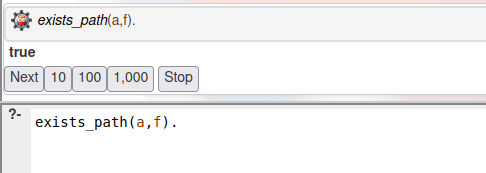
\includegraphics[width=0.9\textwidth]{images/ex2_output}
    		\caption{\code{exists\textunderscore path} query in Exercise 2.}
    	\end{minipage}
    \end{figure}

    \newpage
    
    \begin{Exercise}Define a \code{predicate\textunderscore path/3} which will return a list of nodes (i.e. the path) starting from the initial node to the final node. For example, the following question would result in multiple answers:
    	\code{?- path(a, f, Route). \\
    		Route=[a, b, c, f]; \\
    		Route=[a, b, d, e, f]; \\
    		Route=[a, b, d, c, f]; \\
    		...} \\
    	
    \end{Exercise}

    \textbf{Solution} \\
    
    To construct the predicates for this exercise we are using both the \code{member}, and \code{dif} predicates as a helping hand:  
    
    \begin{lstlisting}[language=Prolog]
%path/3
path(StartNode, EndNode, Route) :- path(StartNode, EndNode, [], Route).
    	
path(StartNode, StartNode, _, [StartNode]).
    	
path(StartNode, EndNode, VisitedNodes, [StartNode|Nodes]) :-
    \+ member(StartNode, VisitedNodes), %member/2 is true if StartNode is member of VisitedNodes list
    dif(StartNode, EndNode), %dif/2 predicate is true if-f StartNode and EndNode are different
    interconnected(StartNode, Node),
    path(Node, EndNode, [StartNode|VisitedNodes], Nodes).
    \end{lstlisting}

    \begin{figure}
    	\centering
    	\begin{minipage}{0.55\textwidth}
    		\centering
    		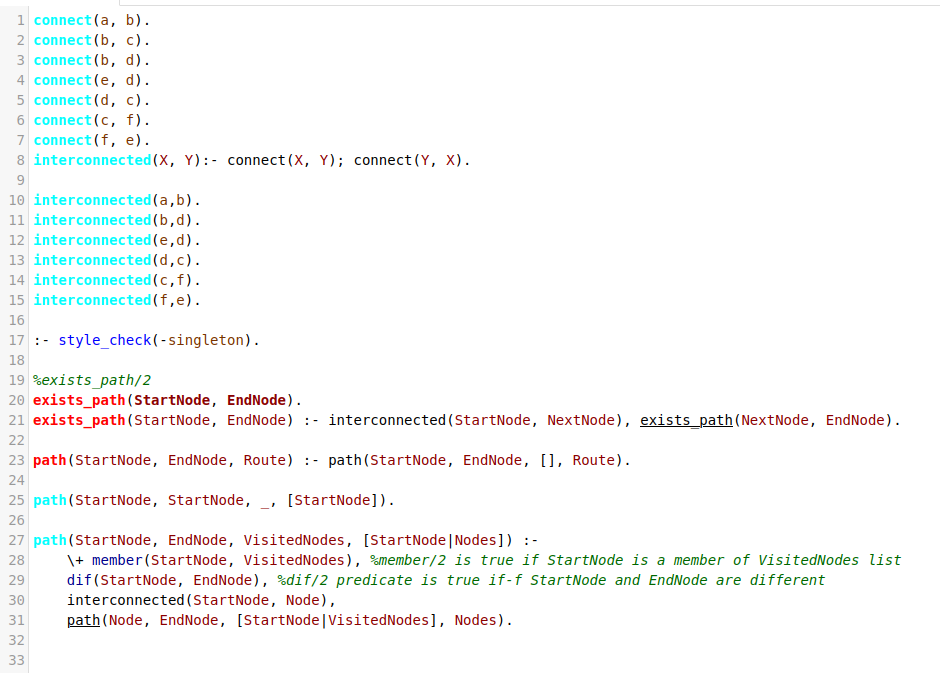
\includegraphics[width=0.9\textwidth]{images/ex3_input} 
    		\caption{KB and rules in Exercise 3.}
    	\end{minipage}\hfill
    	\begin{minipage}{0.45\textwidth}
    		\centering
    		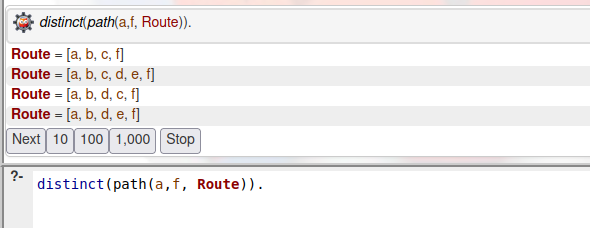
\includegraphics[width=0.9\textwidth]{images/ex3_output} 
    		\caption{\code{path(StartNode, EndNode, Route)} query in Exercise 3. Query returns multiple routes as answers.}
    	\end{minipage}
    \end{figure}
    
    \newpage
    
    \begin{Exercise}Consider the weighted graph shown in Figure 3 where each edge has a specific cost. Modify the facts so that they include the cost information as shown below: \\
    	\code{
    	connect(a, b, 3). \\
    	connect(b, c, 12). \\
    	connect(b, d, 4). \\
    	...}
    
    \begin{wrapfigure}{r}{0.2\textwidth}
    	\begin{center}
    		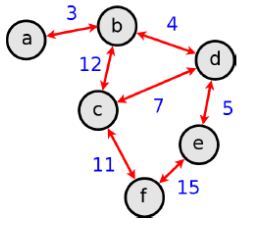
\includegraphics[width=0.25\textwidth]{images/fig2.png}
    	\end{center}
    	\caption{A weighted graph.}
    \end{wrapfigure}

    and the rules: \\
    \code{interconnected(X, Y, C):- connect(X, Y, C). \\
    interconnected(X, Y, C):- connect(Y, X, C).} \\

    Define a predicate \code{cost\textunderscore path/4}, which will return a list of nodes starting from the initial node to the final node (like the previous task 3) and the total cost of the path.
    The total cost of the route should be calculated at the same time as finding it. For example, the following question would result in multiple answers: \\
    
    \code{?- cost\textunderscore path(a, f, Route, Cost). \\
    	Route=[a, b, d, c, f], \\
    	Cost=25; \\
    	Route=[a, b, c, f], \\
    	Cost=26; \\
    	...}
    \end{Exercise}

    \textbf{Solution} \\
    
    The solution in this exercise is very similar to the previous one, using a list to keep track of the visited nodes and using the \code{member} and \code{dif} predicates, autoloated from \code{swi-prolog}. \\
    
     \begin{figure}
    	\centering
    	\begin{minipage}{0.55\textwidth}
    		\centering
    		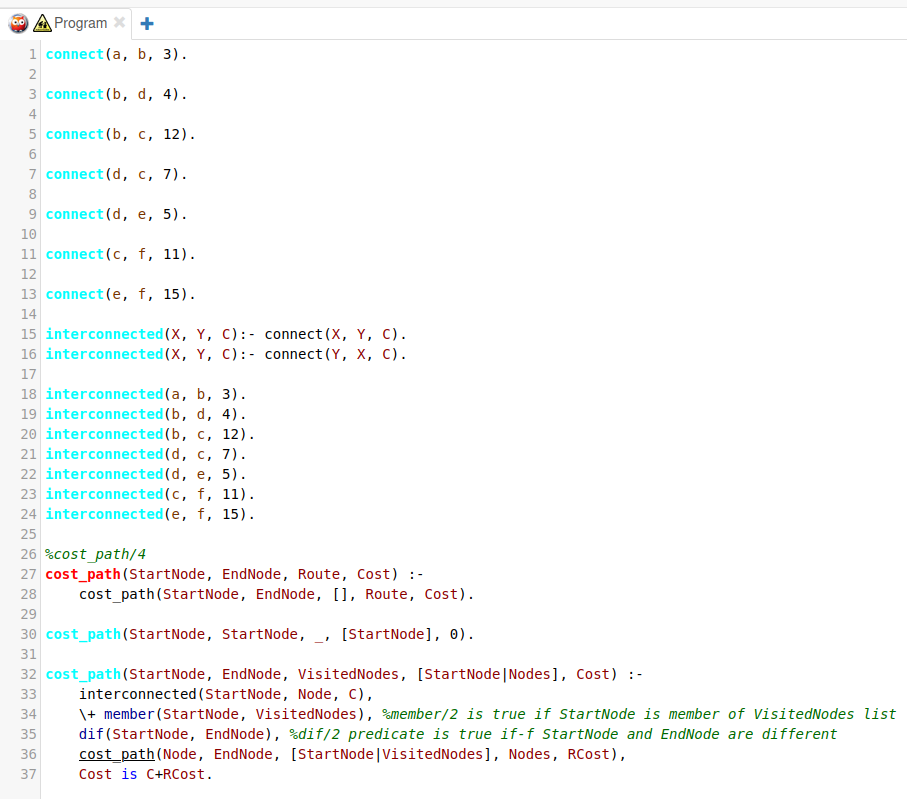
\includegraphics[width=0.9\textwidth]{images/ex4_input} % first figure itself
    		\caption{KB and rules for Exercise 4.}
    	\end{minipage}\hfill
    	\begin{minipage}{0.45\textwidth}
    		\centering
    		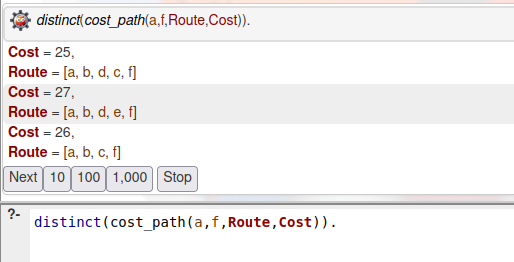
\includegraphics[width=0.9\textwidth]{images/ex4_output} % second figure itself
    		\caption{\code{cost\textunderscore path(StartNode, EndNode, Route, Cost)} query for Exercise 4. Query returns multiple paths and their associated costs as answers.}
    	\end{minipage}
    \end{figure}

   \begin{lstlisting}[language=Prolog]
%cost_path/4
cost_path(StartNode, EndNode, Route, Cost) :-
    cost_path(StartNode, EndNode, [], Route, Cost).

cost_path(StartNode, StartNode, _, [StartNode], 0).

cost_path(StartNode, EndNode, VisitedNodes, [StartNode|Nodes], Cost) :-
    interconnected(StartNode, Node, C),
    \+ member(StartNode, VisitedNodes), %member/2 is true if StartNode is member of VisitedNodes list
    dif(StartNode, EndNode), %dif/2 predicate is true if-f StartNode and EndNode are different
    cost_path(Node, EndNode, [StartNode|VisitedNodes], Nodes, RCost),
    Cost is C+RCost.
    \end{lstlisting}


Complete Prolog code listing of Assignment \# 4 is available on the Appendix, located at the next page.

\newpage

\section{Appendix}

\appendix

\begin{lstlisting}[language=Prolog, caption=Complete Code Listing]
%%%%%%%%%%%%%%%%%%%%%%%%%%%%%%%%%%%%%%%%%
%%%%%%%%%%%%%   Homework 4  %%%%%%%%%%%%%
%%%%%%%%%%%%%%%%%%%%%%%%%%%%%%%%%%%%%%%%%
%%%% CS-487 Fall Semester 2022-2023  %%%%
%%%% Department of Computer Science  %%%%
%%%%       University of Crete       %%%%
%%%%%%%%%%%%%%%%%%%%%%%%%%%%%%%%%%%%%%%%%
%% Nikolaos-Modestos Kougioulis (1285) %%
%%%%%%%%%%%%%%%%%%%%%%%%%%%%%%%%%%%%%%%%%

connect(a, b).

connect(b, c).

connect(b, d).

connect(e, d).

connect(d, c).

connect(c, f).

connect(f, e).

%interconnected(X, Y):- connect(X, Y).
%interconnected(X, Y):- connect(Y, X).
interconnected(X, Y):- connect(X, Y); connect(Y, X).

interconnected(a,b).
interconnected(b,d).
interconnected(e,d).
interconnected(d,c).
interconnected(c,f).
interconnected(f,e).

:- style_check(-singleton).

%exists_path/2
%exists_path(StartNode, EndNode).
%exists_path(StartNode, EndNode) :- connect(StartNode, NextNode), exists_path(NextNode, EndNode).

%exists_path/2 with interconnect
exists_path(StartNode, EndNode).
exists_path(StartNode, EndNode) :- interconnected(StartNode, NextNode), exists_path(NextNode, EndNode).

%path/3
path(StartNode, EndNode, Route) :- path(StartNode, EndNode, [], Route).

path(StartNode, StartNode, _, [StartNode]).

path(StartNode, EndNode, VisitedNodes, [StartNode|Nodes]) :-
    \+ member(StartNode, VisitedNodes), %member/2 is true if StartNode is member of VisitedNodes list
    dif(StartNode, EndNode), %dif/2 predicate is true if-f StartNode and EndNode are different
    interconnected(StartNode, Node),
    path(Node, EndNode, [StartNode|VisitedNodes], Nodes).

connect(a, b, 3).

connect(b, d, 4).

connect(b, c, 12).

connect(d, c, 7).

connect(d, e, 5).

connect(c, f, 11).

connect(e, f, 15).

interconnected(X, Y, C):- connect(X, Y, C).
interconnected(X, Y, C):- connect(Y, X, C).

interconnected(a, b, 3).
interconnected(b, d, 4).
interconnected(b, c, 12).
interconnected(d, c, 7).
interconnected(d, e, 5).
interconnected(c, f, 11).
interconnected(e, f, 15).

%cost_path/4
cost_path(StartNode, EndNode, Route, Cost) :-
    cost_path(StartNode, EndNode, [], Route, Cost).

cost_path(StartNode, StartNode, _, [StartNode], 0).

cost_path(StartNode, EndNode, VisitedNodes, [StartNode|Nodes], Cost) :-
    interconnected(StartNode, Node, C),
    \+ member(StartNode, VisitedNodes), %member/2 is true if StartNode is member of VisitedNodes list
    dif(StartNode, EndNode), %dif/2 predicate is true if-f StartNode and EndNode are different
    cost_path(Node, EndNode, [StartNode|VisitedNodes], Nodes, RCost),
    Cost is C+RCost.
\end{lstlisting}

\end{document}
